\chapter{Inputs to Dakota}\label{input}

\section{Overview of Inputs}\label{input:overview}

Dakota supports a number of command-line arguments, as described in
Section~\ref{tutorial:installation:running}.  Among these are
specifications for the Dakota input file and, optionally, a restart
file.  The syntax of the Dakota input file is described in detail in
the Dakota Reference Manual~\cite{RefMan}, and the restart file is
described in Chapter~\ref{restart}.

A Dakota input file may be prepared with a text editor such as Emacs,
Vi, or WordPad, or with the Dakota graphical user interface.
The Dakota GUI is built on the Java-based Eclipse Framework
\cite{Eclipse} and presents the Dakota input specification options in
synchronized text-editing and graphical views.  The Dakota GUI includes
templates and wizards for helping create Dakota studies and can invoke
Dakota to run an analysis.  The Dakota GUI for Linux, Windows, and
Mac, is available for download from the Dakota website
\url{http://dakota.sandia.gov/}, along with licensing information,
separate GUI documentation, and installation tips.

\subsection{Tabular Data Formats}\label{input:tabularformat}

The Dakota input file and/or command line may identify additional text
files for tabular data import in contexts described in
Section~\ref{input:import}.  Examples include data from which to build
a surrogate, points at which to run a list parameter study, post-run
input data, and least squares and Bayesian calibration data. Dakota
writes and reads tabular data with C++ stream operators/conversions,
so most integer and floating point formats are acceptable for imported
numeric data.  Dakota supports the following tabular formats:
\begin{itemize}

\item \textbf{Annotated:} In most contexts, Dakota tabular data
  defaults to ``annotated'' tabular format.  An annotated tabular file
  is a whitespace-separated text file with one leading header row of
  comments/column labels.  In most imports/exports, each subsequent
  row contains an evaluation ID and interface ID, followed by data for
  variables, or variables followed by responses, depending on context.
  This example shows 5 variables, followed by the 1 text\_book
  response:
\begin{footnotesize}
\begin{verbatim}
%eval_id interface     TF1ln     TF1ln    hpu_r1    hpu_r2 ModelForm      text_book 
1               I1   0.97399    1.0476        12     4.133         3     14753 
2               I1   0.94468    1.0636     4.133        12         3     14753 
3               I1    1.0279    1.0035        12     4.133         3     14753  
\end{verbatim}
\end{footnotesize}
Another example is shown in Figure~\ref{output:tabcont}. \emph{{\bf
    Note:} Dakota 6.1 and newer include a column for the interface ID.
  See the discussion of custom-annotated format for
  importing/exporting Dakota 6.0 format files.}

  For scalar experiment data files, each subsequent row contains an
  experiment ID, followed by data for configuration variables,
  observations, and/or observation errors, depending on context.  This
  example shows 3 data points for each of two experiments.
\begin{verbatim}
%experiment d1 d2 d3
1	82	15.5	2.02
2	82.2	15.45	2
\end{verbatim}

\item \textbf{Free-form:} When optionally specifying \texttt{freeform}
  for a given tabular import, the data file must be provided in a
  free-form format, omitting the leading header row and ID
  column(s). The raw num\_rows x num\_cols numeric data entries may
  appear separated with any whitespace including arbitrary spaces,
  tabs, and newlines.  In this format, vectors may therefore appear as
  a single row or single column (or mixture; entries will populate the
  vector in order).  This example shows the free-form version of the
  annotated data above:
\begin{verbatim}
   0.97399    1.0476        12     4.133         3     14753 
   0.94468    1.0636     4.133        12         3     14753 
    1.0279    1.0035        12     4.133         3     14753 
\end{verbatim}

\item \textbf{Custom-annotated:} In Dakota 6.2 and newer, a
  custom-annotated format is supported, to allow
  backward-compatibility with Dakota 6.0 tabular formats, which had a
  header and evaluation ID, but no interface ID.  This can be
  specified, for example, with
\begin{verbatim}
method
  list_parameter_study
    import_points_file = 'dakota_pstudy.3.dat'
      custom_annotated header eval_id
\end{verbatim}
  The \texttt{custom\_annotated} keyword has options to control
  \texttt{header} row, \texttt{eval\_id} column, and
  \texttt{interface\_id} column.

\end{itemize}

In tabular files, variables appear in input specification order as
documented in the reference manual.  As of Dakota 6.1, tabular I/O has
columns for all of the variables (active and inactive), not only the
active variables as in previous versions.  To import data
corresponding only to the active variables, use the keyword
\texttt{active\_only} when specifying the import file.

{\bf Attention:} Prior to October 2011, samples, calibration, and
surrogate data files were free-form format.  They now default to
annotated format, though there are {\tt freeform} and {\tt
  custom\_annotated} options.  For both formats, a warning will be
generated if a specific number of data are expected, but extra is
found and an error generated when there is insufficient data.  Some
TPLs like SCOLIB and JEGA manage their own file I/O and only support
the free-form option.


\section{Data Imports}\label{input:import}

The Dakota input file and/or command line may identify additional
files used to import data into Dakota.

\subsection{AMPL algebraic mappings: stub.nl, stub.row, and stub.col}

As described in Section~\ref{advint:algebraic}, an AMPL
specification of algebraic input-to-output relationships may be
imported into Dakota and used to define or augment the mappings of a
particular interface.

\subsection{Genetic algorithm population import}

Genetic algorithms (GAs) from the JEGA and SCOLIB packages support a
population import feature using the keywords
\texttt{initialization\_type flat\_file = \emph{STRING}}.  This is
useful for warm starting GAs from available data or previous runs.
Refer to the Method Specification chapter in the Dakota Reference
Manual~\cite{RefMan} for additional information on this specification.
The flat file must be in free-form format as described in
Section~\ref{input:tabularformat}.

\subsection{Calibration data import}\label{input:calib_data}

%Deterministic least squares and Bayesian Calibration methods allow
%specification of experimental observations to difference with
%responses in calculating a model misfit metric (such as a sum of
%squared residuals). 

Deterministic least squares and Bayesian calibration methods allow 
specification of model misfit metrics (such as a sum of squared residuals) 
to describe the discrepancies between experimental observations and model 
responses.

For scalar responses, a simple tabular format is allowed.  The default
file format is {\tt annotated}, but the {\tt freeform} option is
supported.  The data file is comprised of one or more experiments,
each with one or more replicates, one row per replicate.  The columns
of the data file contain, in sequence,
\begin{itemize}
\item {\bf configuration variables (optional):} state variable values
  indicating the configuration at which this experiment was conducted;
  length must agree with the number of state variables active in the
  study.
\item {\bf experimental observations (required):} experimental data
  values to difference with model responses; length equal to the number 
  of responses.
\item {\bf experimental standard deviations (optional):} measurement
  errors (standard deviations) associated with the experimental observations; 
  one scalar value may be specified for each of the responses.
\end{itemize}

Data informing field-valued responses are input using a separate file
per response group, per experiment.  Field responses may optionally
have scalar, diagonal, or matrix-valued error covariance information.
See~\ref{nls:examples} and the Dakota Reference Manual Responses
section for further details.

As an example, Figure~\ref{fig:input:obs_err_cov} shows an observation
vector with 5 responses; 2 scalar + 3 field (each field of length
\textgreater 1).  The corresponding covariance matrix has scalar
variance for each of the scalars, diagonal covariance for field 1,
scalar covariance for field 2, and full matrix covariance for field 3.
In total, Dakota supports block diagonal covariance $\Sigma$ across
the responses, with blocks $\Sigma_i$, which could be fully dense
within a given field response group.  Covariance across the
highest-level responses (off-diagonal blocks) is not supported.
\begin{figure}[htbp!]
  \centering
  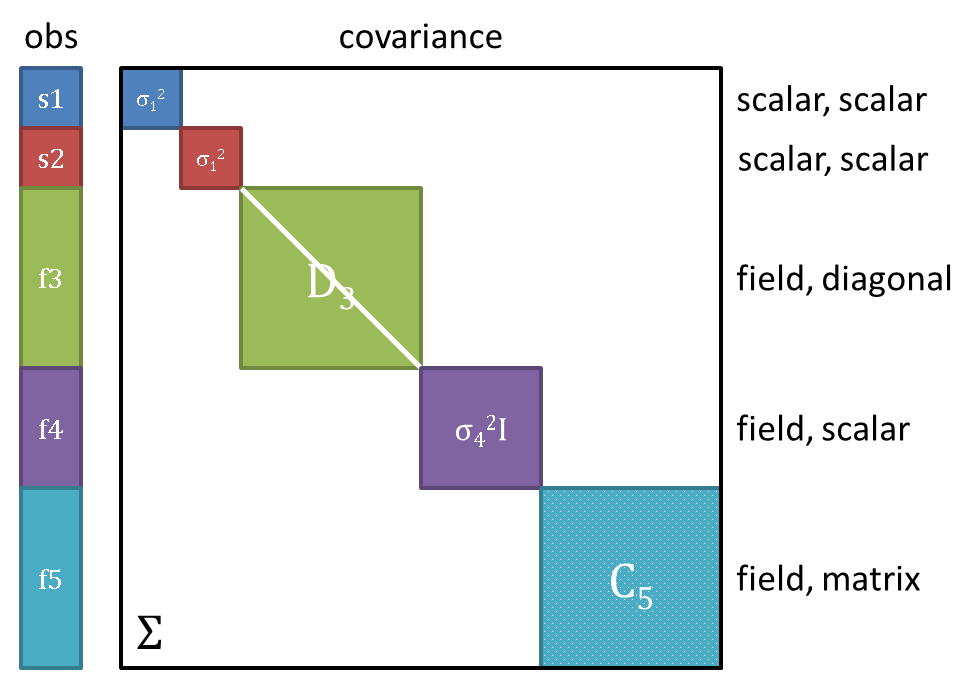
\includegraphics[scale=0.5]{images/ObsErrorCovariance}
  \caption{An example of scalar and field response data, with
    associated block-diagonal observation error covariance.}
  \label{fig:input:obs_err_cov}
\end{figure}

\subsection{PCE coefficient import}

Polynomial chaos expansion (PCE) methods compute coefficients for
response expansions which employ a basis of multivariate orthogonal
polynomials.  Normally, the \texttt{polynomial\_chaos} method
calculates these coefficients based either on a spectral projection or
a linear regression (see Section~\ref{uq:expansion}).  However, Dakota
also supports the option of importing a set of response PCE
coefficients from a file specified with \\
\texttt{import\_expansion\_file = \emph{STRING}}.  Each row of the
free-form formatted file must be comprised of a coefficient followed
by its associated multi-index (the same format used for output
described in Section~\ref{sec:output:pce}).  This file import can be
used to evaluate moments analytically or compute probabilities
numerically from a known response expansion.  Refer to the Method
Specification chapter in the Dakota Reference Manual~\cite{RefMan} for
additional information on this specification.

\subsection{Surrogate construction and evaluation data}

Global data fit surrogates, including some stochastic expansions, may
be constructed from a variety of data sources.  One of these sources
is an auxiliary data file, as specified by the keyword \texttt{import\
  points\_file = \emph{STRING}}.  The file may be in annotated
(default), custom\_annotated, or free-form format with columns
corresponding to variables and responses.  Surfpack global surrogate
models may also be evaluated at a user-provided file containing
\texttt{challenge\_points}.  Refer to the Model Specification chapter
in the Dakota Reference Manual~\cite{RefMan} for additional
information on this specification.

\subsection{Variables/responses import to post-run}

The post-run mode (supported only for sampling, parameter study, and
DACE methods) requires specification of a file containing parameter
and response data.  Annotated is the default format (see Section
~\ref{input:tabularformat}), where leading columns for evaluation and
interface IDs are followed by columns for variables (active and
inactive by default), then those for responses, with an ignored header
row of labels and then one row per evaluation.  Typically this file
would be generated by executing \texttt{dakota -i dakota.in -pre\_run
  ::variables.dat} and then adding columns of response data to
variables.dat to make varsresponses.dat.  The file is specified at the
command line with:
\begin{small}
\begin{verbatim}
    dakota -i dakota.in -post_run varsresponses.dat::
\end{verbatim}
\end{small}
To import post-run data in other formats, specify \texttt{post\_run}
in the input file instead of at the command-line, and provide a format
option.

% LocalWords:  WordPad pre num whitespace freeform TPLs SCOLIB JEGA AMPL nl GAs
% LocalWords:  PCE multi dakota dat varsresponses Surfpack
